\documentclass[11pt,letterpaper]{article}
\usepackage[utf8]{inputenc}
\usepackage[T1]{fontenc}
\usepackage{mathptmx}
\usepackage[letterpaper,left=1.25in,right=1.25in,top=1.2in,bottom=1.2in,headheight=14pt]{geometry}
\usepackage{microtype}
\usepackage{amsmath,amssymb,amsthm,mathtools,bm}
\usepackage{graphicx,booktabs,array,multirow,float}
\usepackage{xcolor}
\usepackage{enumitem}
\usepackage[labelfont=bf,labelsep=colon,font=small,skip=4pt]{caption}
\usepackage{subcaption}
\usepackage{fancyhdr}
\usepackage{titlesec}
\usepackage{listings}
\usepackage{tikz}
\usetikzlibrary{arrows.meta,positioning,calc}
\usepackage[authoryear,round]{natbib}
\definecolor{linkcol}{HTML}{2B3A8F}
\usepackage[colorlinks=true,linkcolor=linkcol,citecolor=linkcol,urlcolor=linkcol]{hyperref}
\usepackage[capitalise,noabbrev]{cleveref}

\pagestyle{fancy}\fancyhf{}
\lhead{\small Technical report.}
\cfoot{\small\thepage}
\renewcommand{\headrulewidth}{0.5pt}
\setlength{\parskip}{4pt plus 1pt}\setlength{\parindent}{0pt}
\titleformat{\section}{\large\bfseries}{\thesection}{0.8em}{}
\titleformat{\subsection}{\normalsize\bfseries}{\thesubsection}{0.8em}{}
\titleformat{\subsubsection}{\normalsize\bfseries\itshape}{\thesubsubsection}{0.8em}{}
\titlespacing*{\section}{0pt}{16pt}{6pt}\titlespacing*{\subsection}{0pt}{12pt}{4pt}
\setlist{itemsep=1pt,topsep=3pt}
\setlength{\emergencystretch}{2em}

\theoremstyle{definition}
\newtheorem{definition}{Definition}
\theoremstyle{remark}
\newtheorem{remark}{Remark}

\lstset{basicstyle=\ttfamily\small,breaklines=true,frame=single,framerule=0.3pt,
  xleftmargin=4pt,xrightmargin=4pt,columns=fullflexible,keepspaces=true,showstringspaces=false}

% title block: \reporttitle{title}{subtitle}{authors}{affiliation line}
\newcommand{\reporttitle}[4]{%
\begin{center}
{\LARGE\bfseries #1\\[4pt]
\Large #2\par}
\vspace{1.4em}
{\bfseries\color{linkcol}\large #3}\\[0.4em]
{\small #4}\par
\vspace{1.2em}
\end{center}}
\newcommand{\abstractblock}[1]{%
\begin{center}\textbf{Abstract}\end{center}
\vspace{-0.4em}
\begin{quote}\small #1\end{quote}
\vspace{0.4em}}

\begin{document}
\reporttitle{FitPal: Repetition-Level Muscle-Activation Feedback}{Surface EMG on an M5Stack Core2 with Per-User Calibration}{Juan Fernando Castaño \quad Diab Singer \quad Román Villarreal}{Correspondence: \href{mailto:jfc9577@nyu.edu}{jfc9577@nyu.edu}}

\abstractblock{A repetition counter driven by one EMG threshold works for one person on one day. Electrode placement, skin impedance and muscle mass change the amplitude several-fold between users, and mains hum or a knocked cable is enough to produce a count. FitPal is a wearable surface-EMG device that tells a lifter, repetition by repetition, whether the target muscle was actually worked. A Grove EMG sensor feeds an M5Stack Core2, which shows an ``effective'' or ``not effective'' screen, vibrates, and streams results to an Arduino IoT Cloud dashboard. The firmware samples at 1\,kHz in a dedicated FreeRTOS task, applies a 50\,Hz notch and 20--350\,Hz band limits, computes a 100\,ms RMS envelope, expresses it as a fraction of the user's maximum voluntary contraction (\%MVC) measured in a six-second calibration, and detects repetitions with a hysteresis detector and a duration gate. The whole signal chain is one hardware-independent header that is compiled and tested on a PC; its envelope agrees with an independent Python implementation to 0.0076\,mV and both return the same ten repetitions with the same flags. On simulated sessions containing mains hum, DC offset, baseline wander, motion spikes and a $\pm$35\% spread in subject gain, the chain reaches F1\,=\,0.995 over 60 sessions, against 0.563 for a fixed-threshold detector. The signal model is our own, so these scores describe the algorithm and not people. The sketch compiles for the Core2 with the ESP32 Arduino core. Scoring on recordings from the physical sensor, and a run on the device, are still to be done.}

\section{Introduction}
A lifter usually cannot tell whether a repetition loaded the intended muscle. Machines and coaches give indirect cues; surface electromyography (EMG) measures the electrical activity of the muscle itself. The difficulty is that a raw EMG voltage is not a reading. It is a noise-like signal, between tens of microvolts and a few millivolts at the skin, whose \emph{power} follows muscle activation, and it sits on top of a DC offset, baseline wander, mains interference and motion artefacts that are often larger than the signal.

We ask two questions about a small embedded system that turns that voltage into a verdict.

\textbf{Question 1: can the verdict be made independent of the user?} Amplitude differs between people, between electrode placements and between days. A threshold in millivolts is therefore a property of one session. The system has to measure each user's own range and judge every repetition against it.

\textbf{Question 2: how do we know the firmware does what we say it does?} A device on a microcontroller is hard to inspect, and a subject is not always available. We want a procedure in which the code that runs on the board is the code that is tested, and in which the test signal contains the artefacts that break simple detectors.

\textbf{What we find.} Per-user normalisation by a six-second calibration removes the dependence on gain: over 60 simulated sessions with a $\pm$35\% gain spread, the chain finds every effective repetition and miscounts five, while a fixed threshold finds fewer than half of them. The signal chain is a single header with no Arduino dependency, so the same file is built into the firmware and into the PC test; the two agree to 0.0076\,mV. We have not scored real recordings, and the simulation is our own model, so we claim the algorithm is correct and robust to the listed artefacts, nothing more.

\textbf{Contributions.} We do not propose a new EMG method; every stage is standard. The contributions are the following.
\begin{enumerate}
\item A complete embedded chain, from ADC to an effective/not-effective flag, with the reasoning behind each parameter (\cref{sec:system}).
\item A calibration procedure of about six seconds that expresses activation as a fraction of the user's own maximum and fails visibly when the electrode is off or the user does not contract.
\item A firmware structure in which a 1\,kHz sampler task is decoupled from the display and the cloud connection.
\item A verification pipeline in which the device header is compiled on a PC and compared with an independent implementation, plus a simulated evaluation with ground truth (\cref{sec:protocol}).
\item Code, simulation and raw figures in one repository (\cref{app:repro}).
\end{enumerate}

\textbf{Organisation.} \Cref{sec:background} gives background on surface EMG. \Cref{sec:system} describes the hardware and the signal chain, \cref{sec:protocol} the verification protocol, \cref{sec:results} the results, and \cref{sec:discussion} what they do and do not establish.

\section{Background}\label{sec:background}
\textbf{Surface EMG.} The signal recorded over a muscle is the sum of motor-unit action potentials. Its useful energy lies roughly between 20 and 450\,Hz \citep{deluca1997,merletti2004}, and its amplitude, not its instantaneous value, tracks effort. Estimating that amplitude from a short window, for example a moving RMS, is standard practice, and the choice of window and of noise suppression affects the estimate \citep{clancy2002}.

\textbf{Normalisation.} Raw amplitude cannot be compared across people or sessions, so it is usually expressed relative to a reference contraction, most often a maximum voluntary contraction (MVC). The method has known weaknesses, since an MVC depends on motivation and technique, but it remains the common choice for healthy participants \citep{burden2010}. We use it because it needs no equipment beyond the device itself.

\textbf{Interference and electrode practice.} Mains pickup appears as a narrow line at 50 or 60\,Hz; baseline wander and motion artefact sit below about 20\,Hz. Sensor and electrode placement recommendations are collected in the SENIAM guidelines \citep{hermens2000}. The Core2's ESP32 converter is noisy and nonlinear, which is why we average four reads per sample and use the calibrated millivolt conversion.

\textbf{Fatigue.} A falling peak amplitude across a set is one simple indicator of fatigue; spectral indicators are more specific but need longer windows and more computation \citep{cifrek2009}. We use only the first.

\section{System and Signal Chain}\label{sec:system}
\subsection{Hardware}
The sensor is a Grove EMG module. Its VOUT pin goes to pin G35 of the M5Stack Core2, VCC to 5\,V and GND to GND; the electrodes connect to the module through a TRS plug (\cref{fig:hw}). The Core2 supplies the display, three buttons, a vibration motor and Wi-Fi.
\begin{figure}[t]\centering
\begin{subfigure}{0.36\linewidth}\centering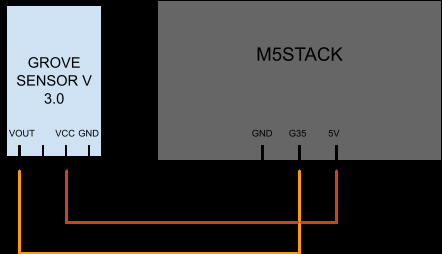
\includegraphics[width=\linewidth]{figures/wiring_diagram.png}\caption{Connections.}\end{subfigure}\hfill
\begin{subfigure}{0.56\linewidth}\centering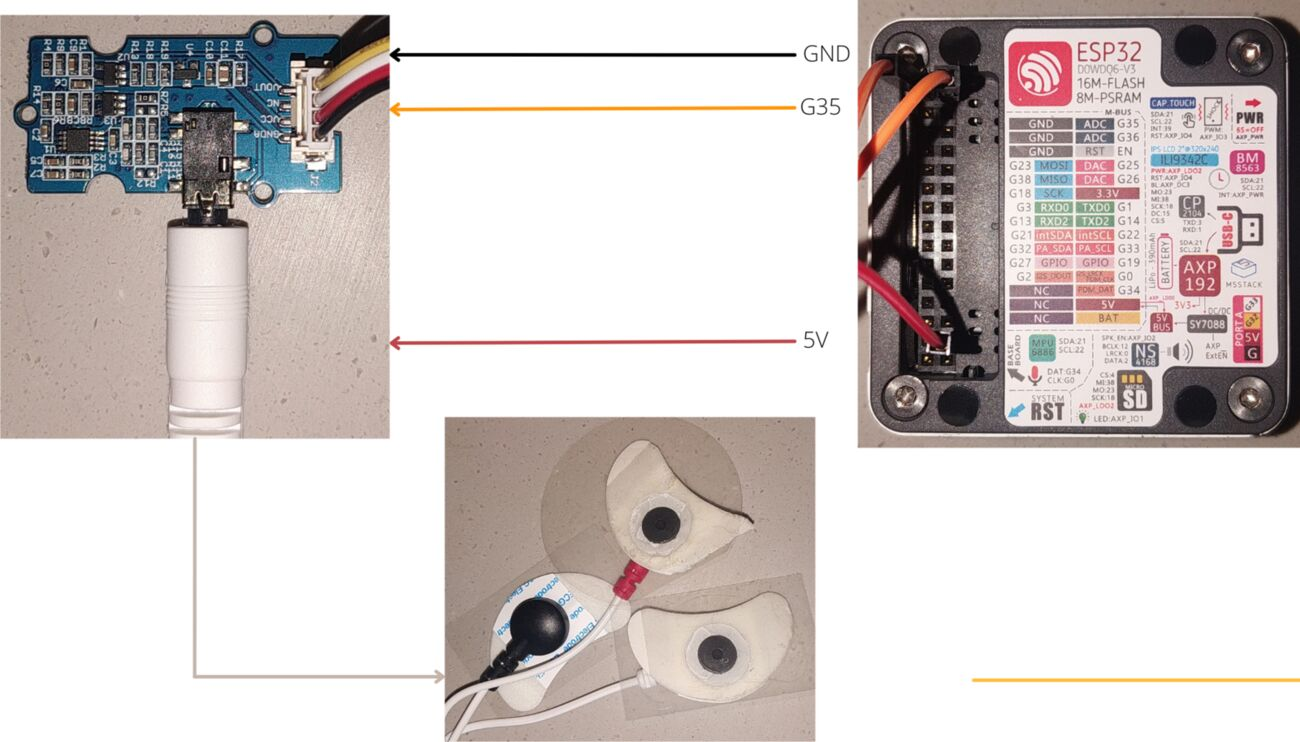
\includegraphics[width=\linewidth]{figures/hardware.jpg}\caption{Sensor, electrodes and Core2.}\end{subfigure}
\caption{Hardware.}\label{fig:hw}
\end{figure}
\begin{figure}[t]\centering
\begin{subfigure}{0.47\linewidth}\centering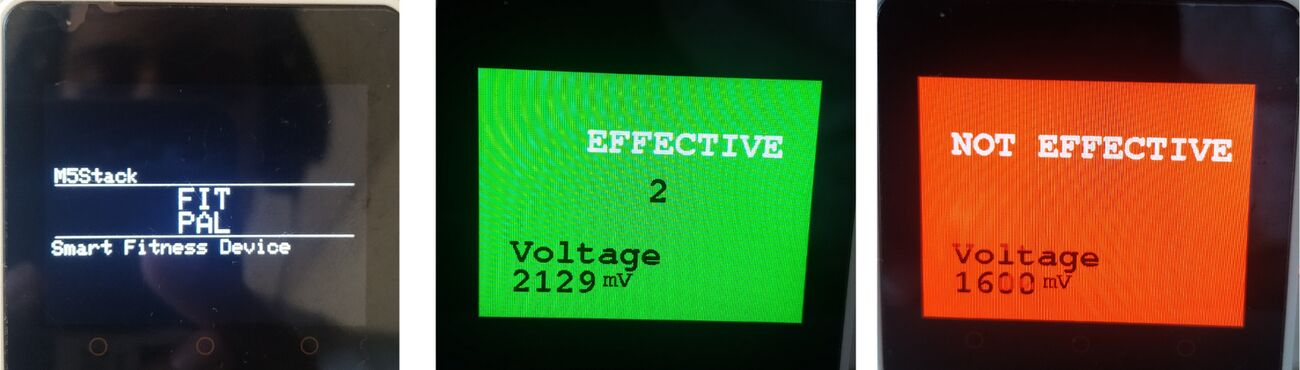
\includegraphics[width=\linewidth]{figures/screens.jpg}\caption{Device screens.}\end{subfigure}\hfill
\begin{subfigure}{0.47\linewidth}\centering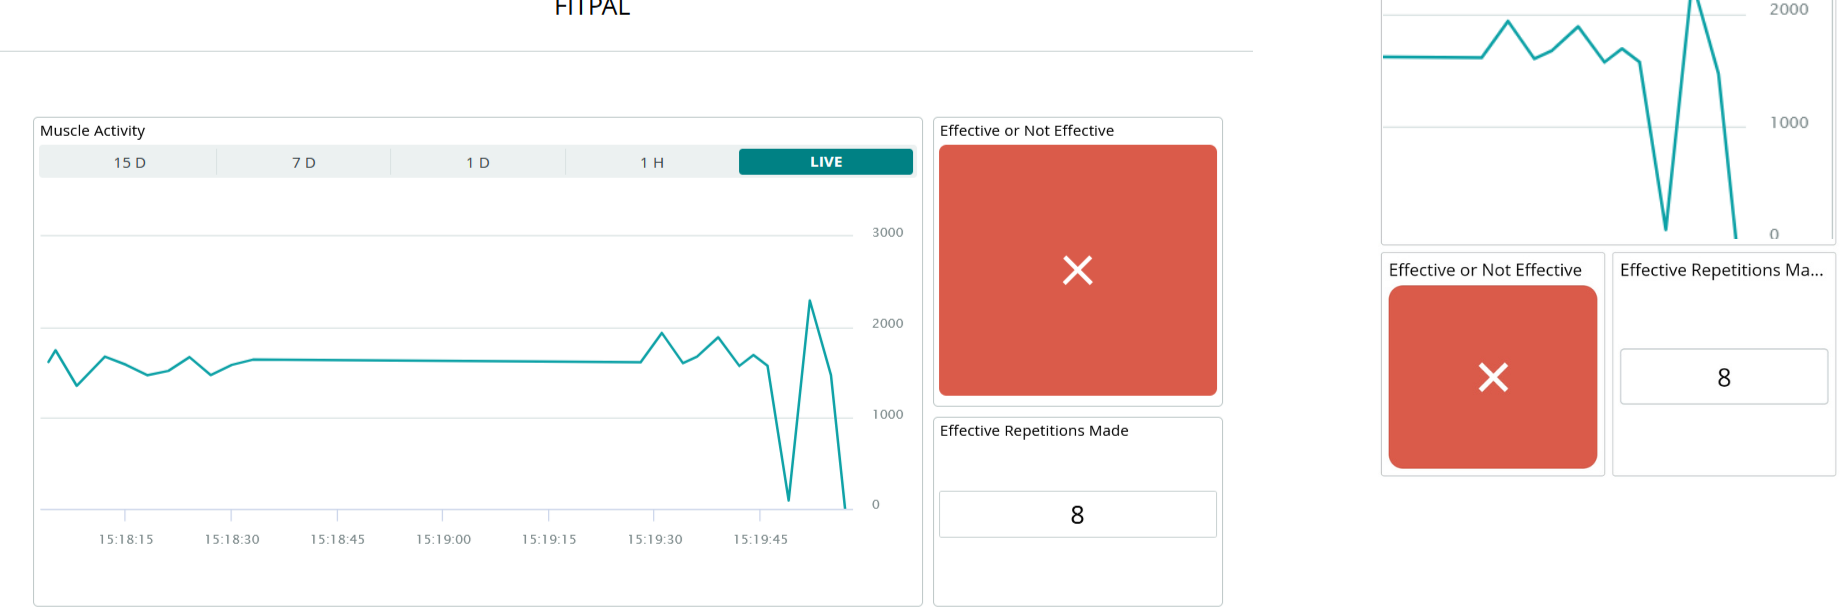
\includegraphics[width=\linewidth]{figures/dashboard.png}\caption{Arduino IoT Cloud dashboard.}\end{subfigure}
\caption{User interface on the device and in the cloud.}\label{fig:ui}
\end{figure}
\begin{figure}[t]\centering
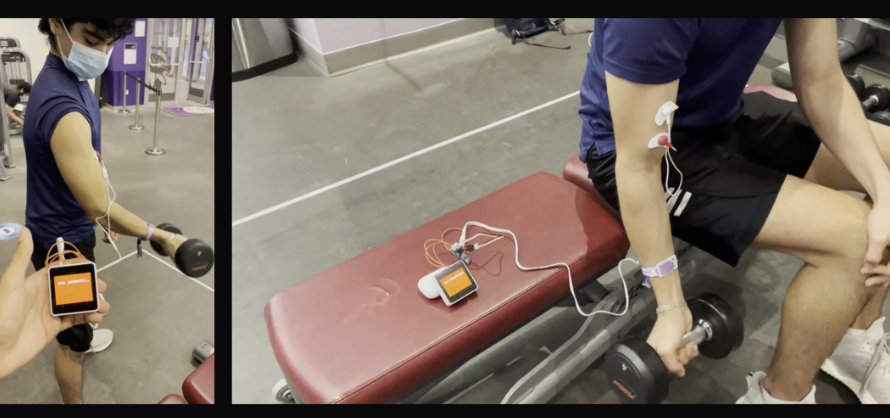
\includegraphics[width=0.92\linewidth]{figures/live-implementation.png}
\caption{The device during a biceps curl: electrodes on the arm, Core2 held in the other hand and resting on the bench. Frames from demonstration footage; this footage is not part of the evaluation in \cref{sec:results}.}\label{fig:live}
\end{figure}

\subsection{Signal chain}
Samples are processed once per millisecond in this order (\cref{fig:chain}).
\begin{figure}[t]\centering
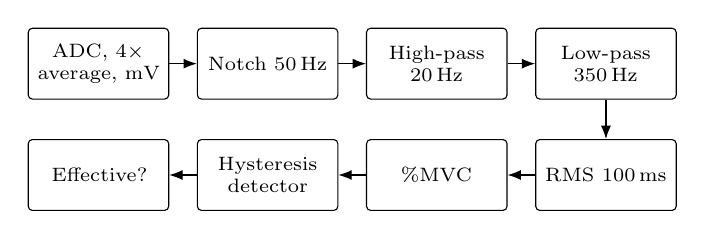
\begin{tikzpicture}[>=Latex,node distance=3.5mm,s/.style={draw,rounded corners=1.5pt,minimum height=9mm,text width=1.55cm,align=center,font=\scriptsize}]
 \node[s] (a) {ADC, $4\times$ average, mV};
 \node[s,right=of a] (b) {Notch 50\,Hz};
 \node[s,right=of b] (c) {High-pass 20\,Hz};
 \node[s,right=of c] (d) {Low-pass 350\,Hz};
 \node[s,below=5mm of d] (e) {RMS 100\,ms};
 \node[s,left=of e] (f) {\%MVC};
 \node[s,left=of f] (g) {Hysteresis detector};
 \node[s,left=of g] (h) {Effective?};
 \draw[->] (a)--(b); \draw[->] (b)--(c); \draw[->] (c)--(d); \draw[->] (d)--(e); \draw[->] (e)--(f); \draw[->] (f)--(g); \draw[->] (g)--(h);
\end{tikzpicture}
\caption{Signal chain from the pin to the repetition verdict.}\label{fig:chain}
\end{figure}

\textbf{Acquisition.} A dedicated FreeRTOS task on core 0 wakes every millisecond with \texttt{vTaskDelayUntil}. Each sample is the mean of four \texttt{analogReadMilliVolts} reads, so every later value is in real millivolts.

\textbf{Mains notch.} A biquad notch with $Q=30$ at the grid frequency (50\,Hz by default; a constant selects 60\,Hz) with coefficients from the audio-EQ cookbook \citep{rbj}. It removes hum without cutting into the EMG band.

\textbf{High-pass, 20\,Hz, and low-pass, 350\,Hz.} Second-order Butterworth sections ($Q=1/\sqrt2$). The high-pass removes the sensor's DC offset, baseline wander and slow motion artefact; the low-pass stays well clear of the 500\,Hz Nyquist limit. Because the high-pass sees the DC offset as a step, the first 500\,ms of data are discarded so the filter settles before any envelope is computed.

\textbf{RMS envelope.} With $x[n]$ the filtered signal and $N=100$ samples (100\,ms),
\begin{equation}
E[n]=\sqrt{\frac{1}{N}\sum_{k=0}^{N-1}x[n-k]^2}.
\end{equation}
It is implemented as a running sum in double precision, so it does not drift over hours at 1\,kHz.

\subsection{Calibration and normalisation}
Pressing A starts a calibration. The user relaxes for 3\,s, which gives the resting envelope $E_{\mathrm{rest}}$ as the mean over the window, then contracts as hard as possible for 3\,s, which gives $E_{\mathrm{MVC}}$ as the maximum. Calibration is accepted only if $E_{\mathrm{MVC}} > 2E_{\mathrm{rest}} + 1$\,mV; otherwise the screen reports a failure, which in practice means an electrode has come off or the user did not squeeze. Activation is then
\begin{equation}
a[n]=\max\!\left(0,\ \frac{E[n]-E_{\mathrm{rest}}}{E_{\mathrm{MVC}}-E_{\mathrm{rest}}}\right).
\end{equation}

\subsection{Repetition detector}
\begin{figure}[t]
\begin{lstlisting}
state IDLE:
    if a >= on and (no previous rep or t - t_end >= 300 ms):
        state = ACTIVE; t0 = t; peak = a
state ACTIVE:
    peak = max(peak, a)
    if a < off or t - t0 > 8 s:
        state = IDLE; t_end = t
        if t - t0 >= 200 ms:
            report rep(start = t0, duration, peak, mean)
            effective = (peak >= target)
\end{lstlisting}
\caption{Repetition detector. Thresholds \texttt{on} and \texttt{off} are 0.30 and 0.15 of MVC for curls (0.28 and 0.14 for squats).}\label{fig:det}
\end{figure}
A repetition starts when $a$ rises above 0.30 and ends when it falls below 0.15; the gap between the two stops the detector chattering around a single level. Bursts shorter than 200\,ms are discarded as artefacts, a 300\,ms refractory period prevents double counting, and an 8\,s limit ends a runaway hold. Each repetition is recorded with its peak, mean and duration, and is \emph{effective} if its peak reaches the exercise target: 0.60 of MVC for curls and 0.54 for squats. These targets are parameters set in \texttt{config.h}, not physiological claims. At the end of a set the device shows the repetition count, the effective count, the mean peak and the least-squares slope of peak against repetition number; a falling slope suggests fatigue.

\subsection{Firmware structure}
The sampler task posts completed repetitions to a queue. The user interface runs on core 1: button A calibrates, B starts and stops a set, C changes exercise. A live activation bar carries a marker at the target; each completed repetition flashes green or red and the motor vibrates for 150\,ms if it was effective. Drawing can take tens of milliseconds without costing a sample. The optional cloud link publishes the activation at 2\,Hz and the two repetition counters when they change; credentials are read from a \texttt{secrets.h} file that is not committed. All of the signal processing is in one header, \texttt{emg\_dsp.h}, with no dynamic allocation and no Arduino dependency.

\section{Verification Protocol}\label{sec:protocol}
\textbf{Parity test.} \texttt{tests/test\_pipeline.cpp} includes \texttt{emg\_dsp.h} unchanged and runs it over a CSV of samples. A Python implementation of the same filter equations, window and detector, written separately, runs on the same file. We compare the envelopes sample by sample and the detected repetitions with their flags.

\textbf{Simulated sessions.} Each session lasts under a minute: 3\,s of rest, two maximal contractions, then ten repetitions of which two are deliberately weak and must not count as effective, so there are eight effective repetitions per session. The EMG is band-limited noise (20--450\,Hz) whose amplitude follows a smooth activation envelope with a slow decay over the set. We add 50\,Hz hum at 20--100\% of the signal level, a 1.65\,V DC offset, baseline wander, ADC noise and three 80\,ms motion spikes of up to 700\,mV in the exercise window. Subject gain is drawn log-normally with a spread of about 35\%.

\textbf{Comparison detector.} The simplest alternative is a fixed threshold: a repetition is counted when one raw sample exceeds a fixed level, followed by a 600\,ms lock-out. We set the level, 2.37\,V at the ADC pin, by hand for a nominal subject of gain 1.

\textbf{Scoring.} A detection is a true positive if it falls within $-300$ to $+1200$\,ms of the start of a not-yet-matched effective repetition. We report precision, recall and F1 over all 60 sessions (480 effective repetitions).

\section{Results}\label{sec:results}
\subsection{Parity}
On the test session the envelopes of the C++ header and the Python reference differ by at most 0.0076\,mV, which is single-precision rounding. Both detectors return the same ten repetitions with the same effective flags.

\subsection{An example session}
\Cref{fig:session} shows one simulated session. The three motion spikes are visible in the raw trace and in the envelope; none is reported as a repetition, because each is shorter than the 200\,ms gate. Both weak repetitions are detected and marked as below target.
\begin{figure}[t]\centering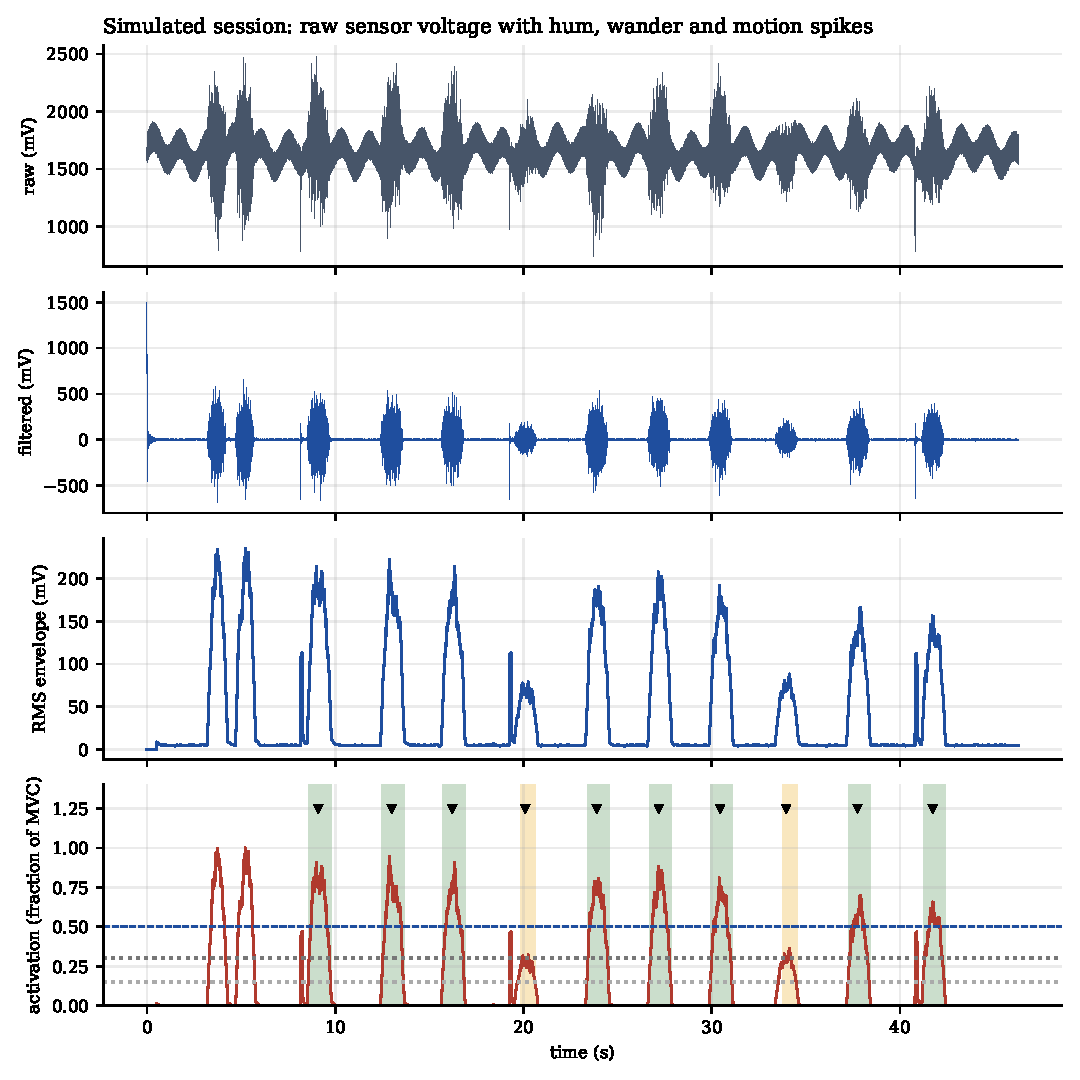
\includegraphics[width=0.86\linewidth]{figures/sim_session.pdf}
\caption{One simulated session. Green bands are effective repetitions and amber bands are detected repetitions below target. Triangles mark ground truth. Dotted lines are the 0.30 and 0.15 thresholds and the dashed line is the 0.50 target used in the simulation.}\label{fig:session}
\end{figure}
\begin{figure}[t]\centering
\begin{subfigure}{0.38\linewidth}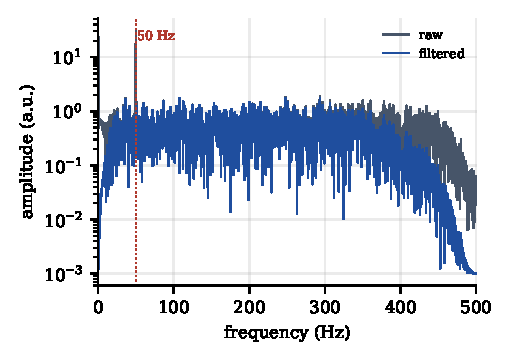
\includegraphics[width=\linewidth]{figures/sim_spectrum.pdf}\caption{Spectrum before and after filtering.}\end{subfigure}\hfill
\begin{subfigure}{0.58\linewidth}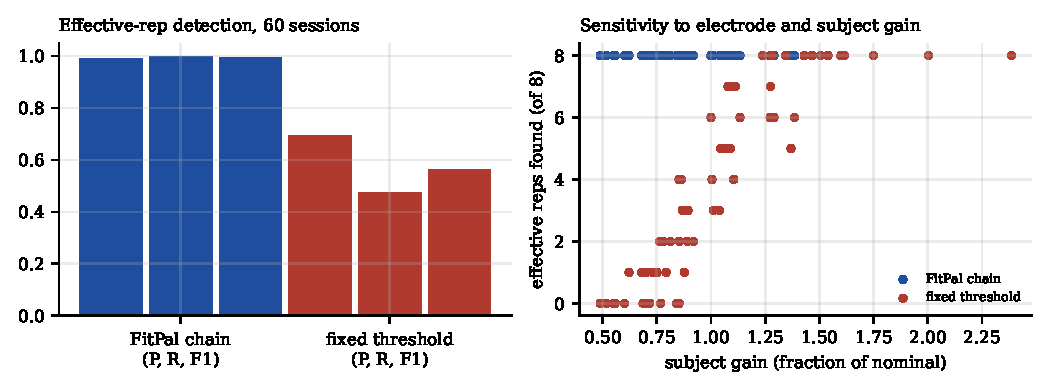
\includegraphics[width=\linewidth]{figures/sim_scores.pdf}\caption{Scores and sensitivity to gain.}\end{subfigure}
\caption{Filter effect and detection performance over 60 simulated sessions.}\label{fig:scores}
\end{figure}

\subsection{Detection over 60 sessions}
\begin{table}[t]\centering\small
\begin{tabular}{@{}lrrrrrr@{}}\toprule
Detector & TP & FP & FN & Precision & Recall & F1\\\midrule
FitPal chain (calibrated, \%MVC) & 480 & 5 & 0 & 0.990 & 1.000 & 0.995\\
Fixed threshold, 600\,ms lock-out & 227 & 100 & 253 & 0.694 & 0.473 & 0.563\\\bottomrule
\end{tabular}
\caption{Effective-repetition detection over 60 simulated sessions with eight effective repetitions each.}\label{tab:scores}
\end{table}
\Cref{tab:scores} gives the totals. The right panel of \cref{fig:scores} explains the gap. The fixed threshold finds none of the effective repetitions at the lowest gains, because the signal never reaches its level, and more of them as gain rises, at which point it starts to count spikes and weak repetitions. The calibrated chain finds all eight at every gain.

\section{Discussion}\label{sec:discussion}
\textbf{Why a fixed threshold fails.} It makes the decision depend on three things the user does not control: electrode placement, skin condition and muscle mass. Hum and spikes then act on top of that. A threshold tuned on one person is correct for that person only. Normalising to a measured maximum moves the unknown out of the decision and into a six-second step the user can repeat when the electrodes are replaced.

\textbf{Practical consequences.} Calibrate again whenever electrodes are repositioned. Set the mains frequency to the local grid. If the Grove module turns out to output an envelope rather than raw EMG, the notch and high-pass stages should be disabled in \texttt{config.h}; the rest of the chain is unchanged.

\textbf{What this study does not establish.} The signal model is ours, so high scores are partly a property of the model. The fixed-threshold detector shows how a threshold behaves when gain varies; it is not a measurement of any existing product. No recordings from the physical sensor have been scored. The sketch compiles for the M5Stack Core2 with ESP32 Arduino core 2.0.17 and the M5Core2 library (about 460\,kB of flash, 25\,kB of static RAM), without the cloud option; the cloud variant was not compiled, and the firmware has not been run on the board. The effectiveness targets of 0.60 and 0.54 of MVC are working values and carry no physiological claim. The fatigue indicator is a slope of peaks and has not been compared with any other measure.

\textbf{Next steps.} Record raw 1\,kHz millivolt streams to SD with video as the reference for repetition count, from several users, both exercises and at least two electrode placements; score detection against the video; measure the stability of $E_{\mathrm{MVC}}$ across days; and run the firmware on the board, including the cloud option.

\textbf{Conclusion.} The device turns a noisy surface-EMG voltage into a per-repetition verdict that is expressed relative to each user's own maximum. The signal chain that runs on the board is the one that was tested, it matches an independent implementation to 0.0076\,mV, and on simulated sessions that include hum, offset, wander, spikes and gain spread it is far more reliable than a fixed threshold. Whether that carries over to people is a question for recorded data.

\section*{Code and data availability}
The firmware, the PC test harness, the simulation and the scripts that generate every figure and number in this report are in the repository accompanying it (\cref{app:repro}).

\bibliographystyle{plainnat}
\bibliography{references}

\appendix
\section{Parameters}
\begin{table}[H]\centering\small
\begin{tabular}{@{}llr@{}}\toprule
Stage & Parameter & Value\\\midrule
Sampling & rate / reads averaged per sample & 1\,kHz / 4\\
Notch & frequency / $Q$ & 50\,Hz (60\,Hz selectable) / 30\\
High-pass, low-pass & corner frequencies & 20\,Hz, 350\,Hz\\
Warm-up & discarded samples & 500\\
Envelope & window & 100\,ms\\
Calibration & rest / maximal contraction & 3\,s / 3\,s\\
Detector & on / off threshold (curl) & 0.30 / 0.15 MVC\\
Detector & minimum duration / refractory / maximum & 200\,ms / 300\,ms / 8\,s\\
Effectiveness & target (curl / squat) & 0.60 / 0.54 MVC\\
Cloud & activation publish rate & 2\,Hz\\\bottomrule
\end{tabular}
\caption{Parameters of the signal chain as set in \texttt{config.h} and \texttt{emg\_dsp.h}.}
\end{table}

\section{Reproducibility}\label{app:repro}
From the repository root, with numpy, scipy, matplotlib and g++ installed:
\begin{lstlisting}
python3 analysis/simulate_and_evaluate.py
\end{lstlisting}
The script builds the C++ test, runs both implementations, writes \texttt{analysis/output/summary.json} and regenerates the three simulation figures. Sessions are seeded, so the numbers in this report are reproduced exactly.
\end{document}
